\documentclass{article}
\usepackage{graphicx}
\graphicspath{ {images/} }
\usepackage[utf8]{inputenc}



\title{Interrupciones a nivel del microprocesador}
\author{Juan Felipe Gutiérrez Sánchez }
\date{Proyecto de investigación - Informática 2}


\begin{document}

\maketitle

\section{¿Qué es una interrupción en el contexto de microprocesadores?}

En el contexto de la informática, especificamente a nivel de microprocesadores, una interrupción es una señal recibida por el procesador de un ordenador, indicando que debe “interrumpir” el curso de ejecución actual y pasar a ejecutar código específico para tratar esta situación.
En pocas palabras una interrupción es una accion del procesador, donde este indica mediante una señal, que algo raro esta sucediendo, y por ende, debe interrumpir la tarea que esta haciendo en el momento, para poder tratar especificamente lo que está pasando para asi poder solucionarlo.
\\[0,5cm]
\section{Historia}
Las interrupciones surgen de las necesidades que tienen los dispositivos periféricos de enviar información al procesador principal de un sistema de computación. Antes de su aparición el primer método que se usó fue que el propio procesador se encargara de sondear (polling) el dispositivo en un lapso de tiempo para averiguar si tenía pendiente alguna información para el. Sin embargo, esta técnica fue ineficiente, ya que el procesador necesitaba de un estimado de tiempo mayor. El mecanismo de interrupciones fue la solución que permitió al procesador desentenderse de esta problemática. En este caso, el microprocesador, no sondea a ningún dispositivo, sino que queda pendiente
de que estos le informen (le "interrumpan").
\\[0.5cm]

\section{Tipos de interrupciones}

Existen 3 diferentes tipos de interrupciones:

\begin{itemize}
\item Interrupciones de HARDWARE: Mecanismo de comunicación entre el procesador y los dispositivos de E/S (Entrada y salida). Sirve para indicar que un dispositivo de E/S tiene datos pendientes de ser tratados. Las interrupciones por hardware evitan que el sistema operativo tenga que muestrear periódicamente el estado de los dispositivos de E/S, de manera que son ellos mismos los que indican que hay datos a ser tratados.
\item Interrupciones de SOFTWARE: Es un mecanismo de comunicación entre un proceso (que se ejecuta en modo usuario) y el sistema operativo (que se ejecuta en modo supervisor). El proceso emplea las interrupciones por software para notificar al sistema operativo que requiere de su intervención.
\item EXCEPCIONES: Las excepciones son otro tipo que emplea el procesador para notificar al sistema operativo de un suceso excepcional, por ejemplo, cuando el proceso realiza la orden div para dividir un valor usando como denominador cero. El tratamiento que generalmente realiza el sistema operativo consiste en terminar con la ejecución del proceso.
\end{itemize}

\section{Implementación interrupciones por HARDWARE}
El controlador envía una petición de interrupción de un solo bit, despues de esto el procesador detecta la señal e identifica la prioridad que tiene, después al aceptar la petición activa una señal de un bit llamada INTA, enviando así al hardware externo el identificador de interrupción para llevar a cabo ese proceso, una vez realizado se envía la señal de vuelta salvando el estado y eliminando la petición del software y posteriormente del hardware que la realizó. Una vez realizado este proceso se restaura el estado en el que se encontraba el procesador y se retoma el programa que se interrumpió
\\[0.5cm]

\section{Implementación interrupciones por SOFTWARE}
Esto solo sucede cuando todos los controladores E/S se conectan al OR-Cableado de la entrada INT de la CPU o si los controladores están conectados en OR a la misma entrada INT. Se lee el registro de cada controlador E/S hasta encontrar el bit de pedido de interrupción para invocar la subrutina asociada a dicho controlador. Debido a la conexión todos se examinan por lo tanto no se deja de atender ningún controlador sin importar que el primero fuese el de la petición. Ell uso del hardware y el tipo del lenguaje es indispensable, ya que depende de la estructura del mismo controlador y el procesador depende de ellos para hacer la interrupción.
\\[0.5cm]
\section{Implementación propia en ARDUINO}
Este es el montaje que decidi hacer en la plataforma TINKERCAD, ya que no se me facilito conseguir el arduino fisico, la interrupción es a nivel de hardware, donde en un principio hay una secuencia de leds, y con un pulsador que está ya montado, este hara que la secuencia cambia hasta que se vuelva a presionar.
attachInterrupt(digitalPinToInterrupt(2),codigo,FALLING);: Esta es la manera que utilice para poder asi crear la interrupción, es la sintaxis propia de arduino, donde hay que ver que tipo de controlador es (en mi caso, ARDUINO UNO), para ver en que entrada es posible hacer la conexion, tambien hay que tener claro que interrupción se va a hacer, en mi caso FALLING, o pin de mayor a menor.

\begin{figure}
\centering
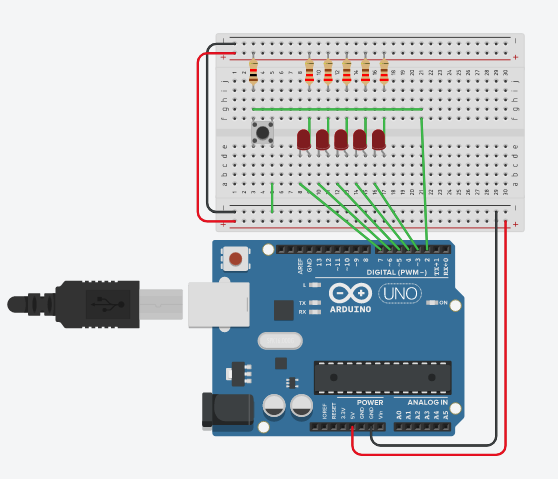
\includegraphics[width=0.50\textwidth]{arduino.png}
\caption{\label{fig1}arduino}
\end{figure}

\section{Fuentes de consulta}

Las siguientes fuentes fueron utilizadas para la consulta:
(Martinez, 2013) Tinoco, J. L. (28 de Marzo de 2011). Slideshare. Obtenido de Interrupciones del microprocesador:https://es.slideshare.net/jorg_leoxd/interrupciones-del-microprocesador

Castellanos, L. (03 de Febrero de 2015). lcsistemasoperativos. Obtenido de Interrupciones:https://lcsistemasoperativos.wordpress.com/tag/interrupciones/

lsi. (05 de Marzo de 2019). Interrupciones y excepciones. Obtenido de Interrupciones y excepciones:https://1984.lsi.us.es/wiki-ssoo/index.php/Interrupciones_y_excepciones

Martinez, Y. (10 de Septiembre de 2013). Youtube. Obtenido de Interrupciones por Hardware y Software:https://www.youtube.com/watch?v=B8ogf7b3A2Q

Universitat Politéecnica de Catalunya, “Hardware del sistema de interrupciones,” Desconocido: http://personals.ac.upc.edu/miguel/materiales/docencia/EC1/material/hardware interrupciones.pdf




\end{document}
